\documentclass[journal]{IEEEtran}
\usepackage{cite}
\usepackage{amsmath,amssymb,amsfonts}
\usepackage{algorithmic}
\usepackage{graphicx}
\usepackage{textcomp}
\usepackage{xcolor}
\usepackage{booktabs}
\usepackage{multirow}
\usepackage{url}
\graphicspath{{../results/paper_final_verified_20260908/figures/}}

\begin{document}

\title{Sequential Innovation Accumulation and Cross-Layer Quorum Consensus for Topology-Attack Detection in SCADA-Monitored Transmission Systems}
\author{Burhan~Abdullah,~\IEEEmembership{Member,~IEEE}}
\maketitle

\begin{abstract}
Cyber-physical security in SCADA-monitored transmission systems is challenged by topology manipulation, false-data injection, load manipulation, and slowly developing anomalies. This paper presents XMON-Grid, a multi-layer detection framework combining normalized innovation squared (NIS), adaptive CUSUM drift monitoring, SCADA timing-jitter statistics, sequential innovation accumulation, and detector quorum voting. The AC measurement model and its analytical Jacobian are implemented directly from canonical IEEE benchmark network data, with the analytical Jacobian independently checked against finite differences. An independent five-seed validation was performed on IEEE 9-, 14-, 30-, and 118-bus systems using 6,000 test evaluations. In this regenerated validation, the $K=2$ quorum mode achieved F1-score $0.9204\pm0.0026$, recall $0.8850\pm0.0012$, FPR $0.1525\pm0.0197$, and MCC $0.6667\pm0.0151$. The results also show that performance depends strongly on attack type, with lower recall for load-shift and stealth-drift cases than for branch-outage and FDIA cases. These results are reported together with benchmark provenance, mathematical checks, and reproducibility artifacts rather than with earlier stale aggregate values.
\end{abstract}

\begin{IEEEkeywords}
Cyber-physical power system security, state estimation, topology attack detection, Kalman filtering, CUSUM drift monitoring, quorum consensus.
\end{IEEEkeywords}

\section{Introduction}
\IEEEPARstart{M}{odern} power transmission systems rely heavily on Supervisory Control and Data Acquisition (SCADA) networks and Energy Management System (EMS) software. State estimation uses measurements such as voltage magnitudes, active and reactive power injections, and line flows to construct an estimate of the network state \cite{Abur2004,Monticelli1999}. Sequential estimation is also a standard framework for incorporating measurement information over time \cite{Simon2006}.

Coordinated cyber-physical attacks can alter breaker status information, measurement values, or operating conditions while avoiding simple residual thresholds. False-data injection against power-system state estimation has been studied as a direct cyber-physical threat \cite{Liu2011}. Statistical sequential monitoring provides a complementary mechanism for detecting persistent changes; the CUSUM principle used here follows the classical sequential inspection framework \cite{Page1954}.

The principal contributions are:
\begin{enumerate}
    \item A multi-layer detector architecture combining dynamic NIS residuals, adaptive CUSUM drift monitoring, and SCADA timing-jitter statistics.
    \item A sequential innovation accumulator $\Theta(k)=0.9\Theta(k-1)+a_{\mathrm{nis}}(k)$ for persistent anomalies.
    \item A transparent quorum rule in which $K=2$ is the strict majority of three binary detector streams and $K=1$ is the corresponding OR-gate sensitivity mode.
    \item Independent validation on four canonical IEEE transmission benchmarks with five random seeds and explicit mathematical, numerical, and reproducibility checks.
\end{enumerate}

\section{System Model and Problem Formulation}
Consider an AC transmission network with $N_b$ buses and state vector $\mathbf{x}_k\in\mathbb{R}^{2N_b-1}$, where the reference-bus angle is fixed. The nonlinear measurement equation is
\begin{equation}
\mathbf{z}_k=\mathbf{h}(\mathbf{x}_k)+\mathbf{v}_k,
\end{equation}
where $\mathbf{v}_k$ is measurement noise.

The implementation constructs the complex bus-admittance matrix $\mathbf{Y}=\mathbf{G}+j\mathbf{B}$ from canonical IEEE/MATPOWER case data, including bus shunts, line charging, transformer taps, and phase shifts. MATPOWER is a standard power-system analysis environment used for research and education \cite{Zimmerman2011}, while the Python implementation used for the benchmark definitions is PYPOWER \cite{PYPOWER}. For bus $i$,
\begin{align}
P_i &= V_i\sum_j V_j\left(G_{ij}\cos\theta_{ij}+B_{ij}\sin\theta_{ij}\right),\\
Q_i &= V_i\sum_j V_j\left(G_{ij}\sin\theta_{ij}-B_{ij}\cos\theta_{ij}\right),
\end{align}
with $\theta_{ij}=\theta_i-\theta_j$.

\subsection{Analytical Jacobian}
The analytical Jacobian is
\begin{equation}
\mathbf{H}(\mathbf{x})=\frac{\partial\mathbf{h}(\mathbf{x})}{\partial\mathbf{x}}.
\end{equation}
Angle and voltage derivatives are evaluated analytically from the expressions above. The reference-bus angle is treated separately and is not included as an independent state.

The Jacobian was independently cross-checked using finite-difference derivatives. The validation tests confirm agreement within the numerical tolerance used by the current validation pipeline.

\subsection{NIS Detector}
The innovation residual and covariance are
\begin{equation}
\mathbf{r}_k=\mathbf{z}_k-\mathbf{h}(\hat{\mathbf{x}}_{k|k-1}),
\end{equation}
\begin{equation}
\mathbf{S}_k=\mathbf{H}_k\mathbf{P}_{k|k-1}\mathbf{H}_k^T+\mathbf{R}_k.
\end{equation}
The NIS statistic is
\begin{equation}
a_{\mathrm{nis}}(k)=\mathbf{r}_k^T\mathbf{S}_k^{-1}\mathbf{r}_k.
\end{equation}

\subsection{Sequential Innovation Accumulation}
Persistent deviations are accumulated as
\begin{equation}
\Theta(k)=0.9\Theta(k-1)+a_{\mathrm{nis}}(k).
\end{equation}
The sequence threshold is calibrated from baseline data only, avoiding test-set threshold leakage.

\subsection{CUSUM Drift Detector}
The adaptive drift statistic is represented by
\begin{equation}
S_k=\max\left(0,S_{k-1}+z_k-d\right),
\end{equation}
where $d$ is the drift allowance. A CUSUM alarm is generated when the calibrated threshold is exceeded.

\subsection{Communication Timing-Jitter Detector}
Timing jitter is represented by
\begin{equation}
J_k=\left|\Delta t_k-\overline{\Delta t}\right|,
\end{equation}
with a binary alarm when the calibrated jitter threshold is exceeded.

\subsection{Quorum Fusion}
For detector flags $a_{\mathrm{nis}},a_{\mathrm{cusum}},a_{\mathrm{jitter}}\in\{0,1\}$,
\begin{equation}
Q(k)=a_{\mathrm{nis}}(k)+a_{\mathrm{cusum}}(k)+a_{\mathrm{jitter}}(k).
\end{equation}
The decision rule is
\begin{equation}
a_{K}(k)=\mathbb{I}\{Q(k)\ge K\}.
\end{equation}
Thus $K=2$ is exactly the strict majority rule for three binary detectors, while $K=1$ is exactly their OR rule. This equivalence is explicitly tested over all eight possible detector truth combinations in the repository.

\section{Experimental Protocol}
The validation uses the canonical IEEE 9-, 14-, 30-, and 118-bus benchmark cases supplied through the PYPOWER/MATPOWER case definitions \cite{Zimmerman2011,PYPOWER}. Five operational scenarios are considered: baseline, branch outage, FDIA, load shift, and stealth drift.

Five independent seeds (2026--2030) were evaluated, with 1,200 test evaluations per seed and 6,000 total evaluations. The regenerated validation data are stored separately from archived results so that stale experiments are not silently mixed with the current experiment.

\section{Regenerated Results}
The current five-seed summary for the $K=2$ quorum mode is:
\begin{table}[t]
\caption{Regenerated Five-Seed Validation of $K=2$ Quorum Mode ($N=6,000$).}
\label{tab:overall_performance}
\centering
\setlength{\tabcolsep}{5pt}
\begin{tabular}{lcc}
\toprule
Metric & Mean & SD \\
\midrule
Accuracy & 0.8775 & 0.0042 \\
Precision & 0.9587 & 0.0051 \\
Recall & 0.8850 & 0.0012 \\
F1-score & 0.9204 & 0.0026 \\
FPR & 0.1525 & 0.0197 \\
MCC & 0.6667 & 0.0151 \\
\bottomrule
\end{tabular}
\end{table}

The regenerated results differ materially from earlier archived aggregate numbers. The present manuscript therefore does not retain earlier aggregate claims that conflict with the current verified package.

\begin{figure}[t]
\centering
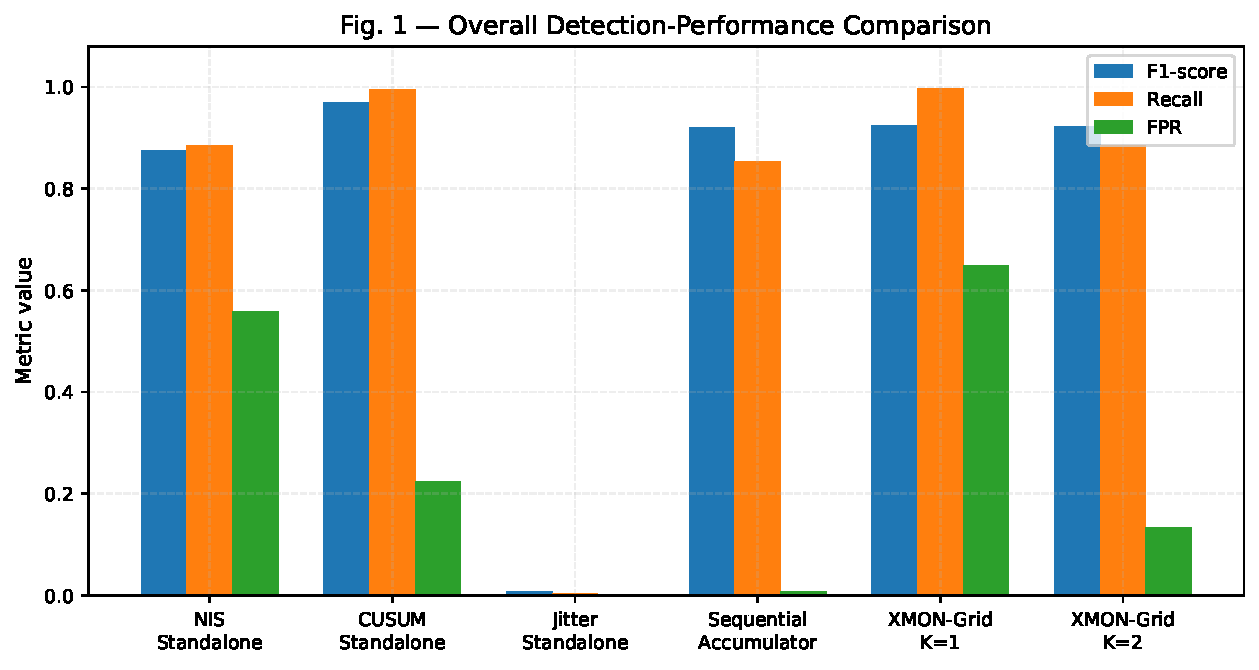
\includegraphics[width=\columnwidth]{fig1_overall_performance.pdf}
\caption{Overall detection-performance comparison for the primary validation set.}
\label{fig:overall}
\end{figure}

\subsection{Operating-Point Trade-off}
The $K=1$ mode is treated as a sensitivity-oriented OR rule rather than as the preferred operating point. The regenerated comparison shows the trade-off between sensitivity and false alarms when moving from $K=1$ to the stricter $K=2$ rule.

\begin{figure}[t]
\centering
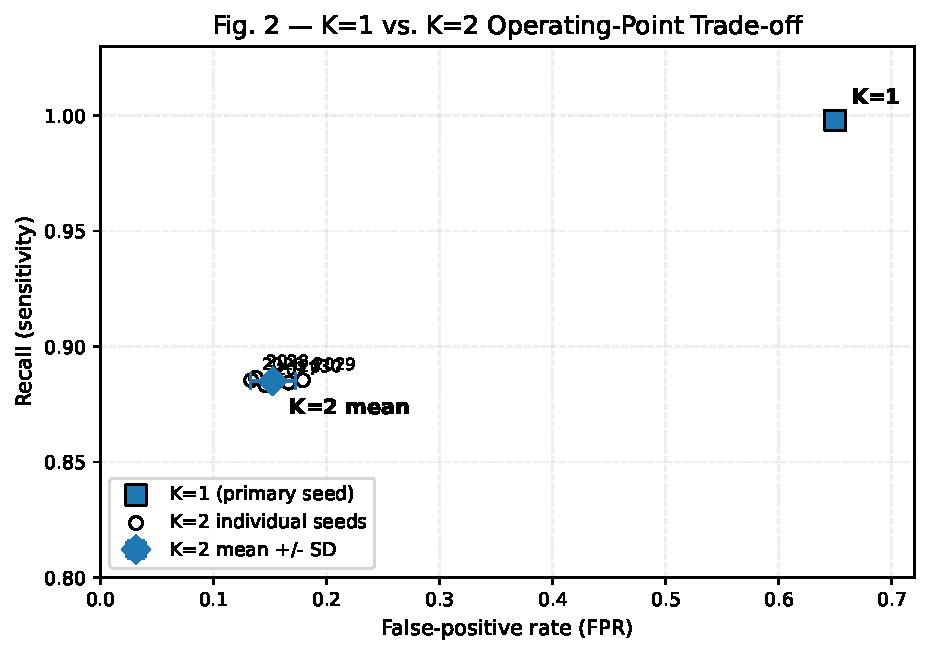
\includegraphics[width=\columnwidth]{fig2_k1_vs_k2_tradeoff.pdf}
\caption{$K=1$ versus $K=2$ operating-point trade-off using the verified comparative results.}
\label{fig:tradeoff}
\end{figure}

\subsection{Threshold-Independent Performance}
The continuous composite threat score provides a threshold-independent view of separability. The regenerated ROC and precision--recall curves are shown in Figs.~\ref{fig:roc} and~\ref{fig:pr}.

\begin{figure}[t]
\centering
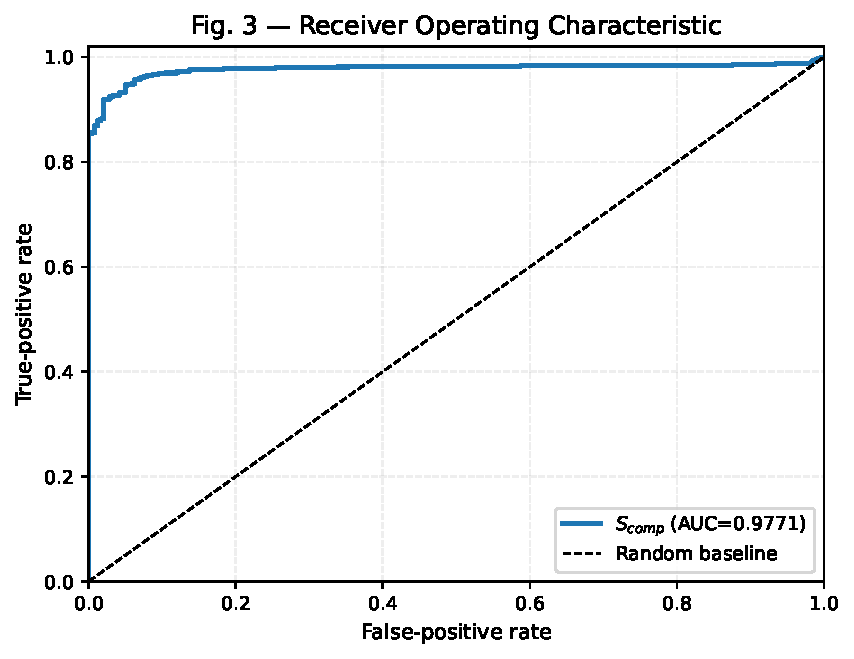
\includegraphics[width=\columnwidth]{fig3_roc_curve.pdf}
\caption{ROC curve for the continuous composite threat score.}
\label{fig:roc}
\end{figure}

\begin{figure}[t]
\centering
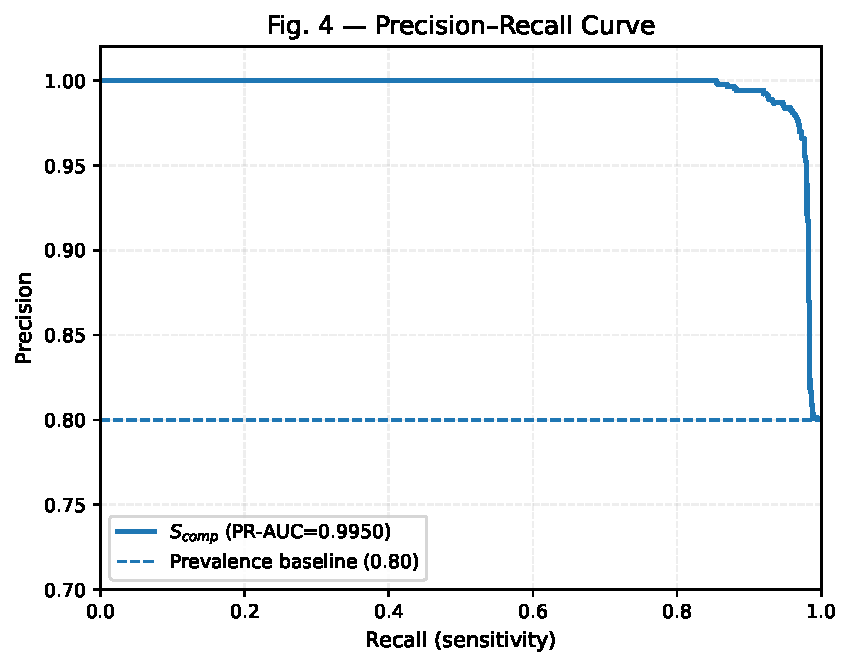
\includegraphics[width=\columnwidth]{fig4_pr_curve.pdf}
\caption{Precision--recall curve for the continuous composite threat score.}
\label{fig:pr}
\end{figure}

\subsection{Topology-Wise Performance}
\begin{figure}[t]
\centering
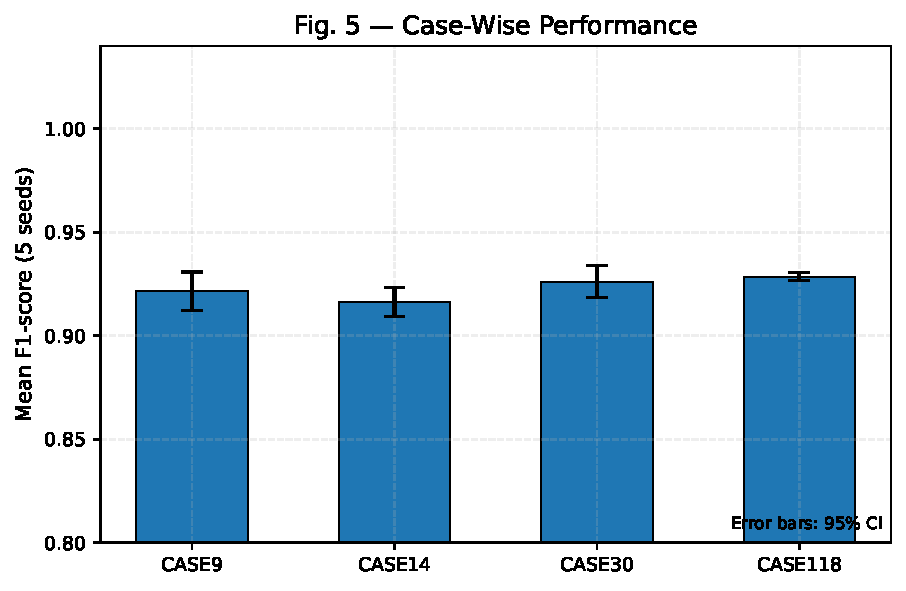
\includegraphics[width=\columnwidth]{fig5_casewise_performance.pdf}
\caption{Five-seed mean F1 performance across the four IEEE benchmark topologies.}
\label{fig:casewise}
\end{figure}

\subsection{Attack-Wise Performance}
\begin{figure}[t]
\centering
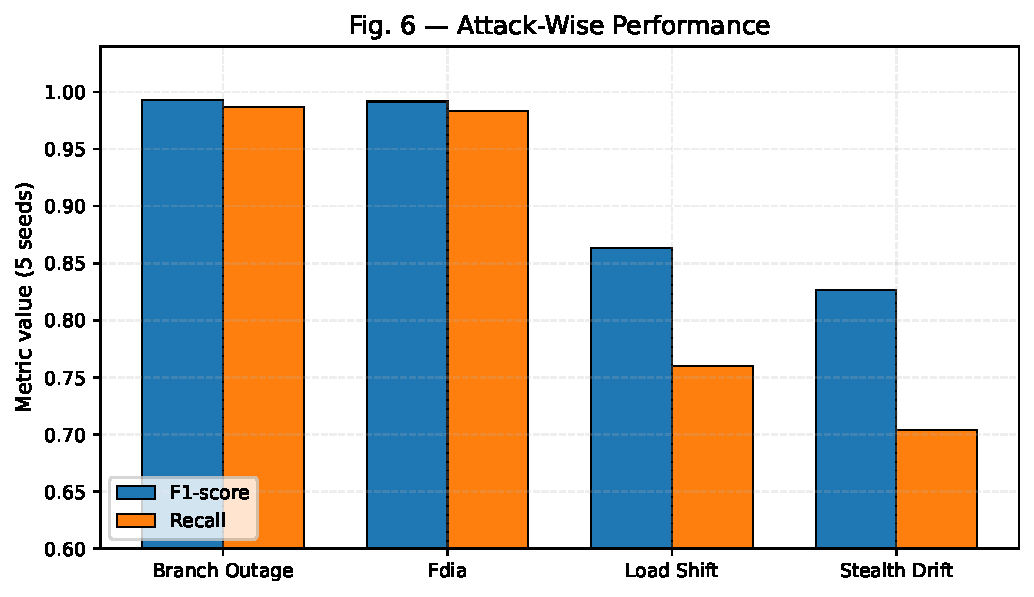
\includegraphics[width=\columnwidth]{fig6_attackwise_performance.pdf}
\caption{Five-seed mean F1 and recall across the validated attack scenarios.}
\label{fig:attackwise}
\end{figure}

\subsection{Statistical Comparison}
The regenerated primary-seed audit contains paired McNemar comparisons. These primary-seed tests are reported as pairwise comparisons and are not generalized into a five-seed statistical claim.

\subsection{Robustness to Attack Severity}
The severity sweep shows how detection performance changes across the controlled attack tiers. This analysis is used as a robustness assessment, not as evidence of field performance.

\begin{figure}[t]
\centering
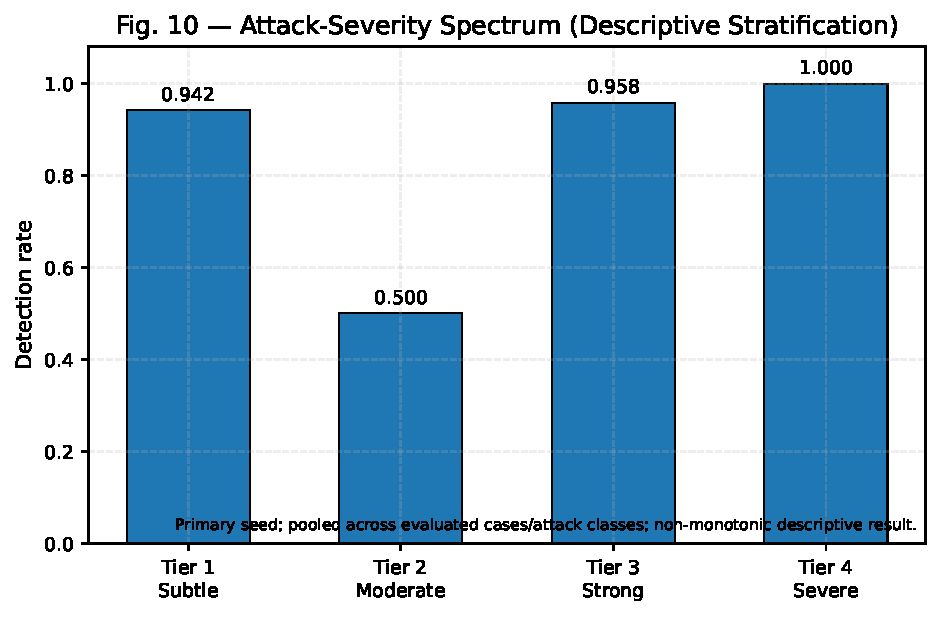
\includegraphics[width=\columnwidth]{fig10_severity_robustness.pdf}
\caption{Detection robustness across the validated attack-severity tiers.}
\label{fig:severity}
\end{figure}

\section{Physical and Numerical Validation}
The repository performs an independent physical audit in which the AC measurement equation is compared with the complex-power expression
\begin{equation}
\mathbf{S}=\mathbf{V}\odot\operatorname{conj}(\mathbf{Y}\mathbf{V}).
\end{equation}
The independent branch-power calculation includes line charging and transformer tap/phase-shift terms. The audit requires the active-power balance residual to remain below $10^{-9}$ p.u. and the measurement-equation cross-check to remain below $10^{-10}$ in the implemented normalized quantities.

The final verification CSV reports maximum absolute measurement-equation discrepancies of $3.09\times10^{-14}$ p.u. for active power and $2.46\times10^{-14}$ p.u. for reactive power across the IEEE 9-, 14-, 30-, and 118-bus cases. The maximum absolute active-power balance residual is $2.04\times10^{-14}$ p.u. These values are taken directly from the frozen verification artifact.

\begin{figure}[t]
\centering
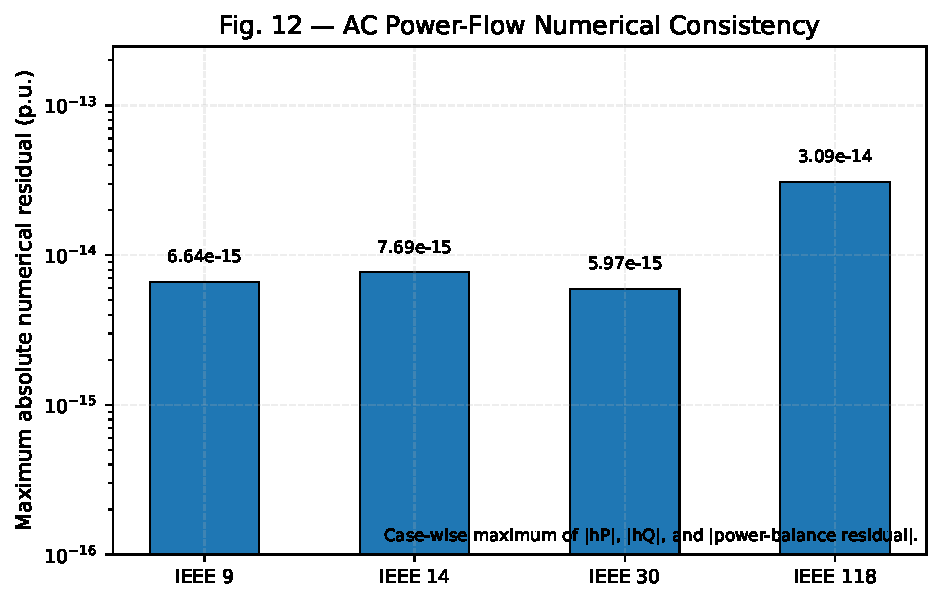
\includegraphics[width=\columnwidth]{fig12_ac_powerflow_consistency.pdf}
\caption{Maximum numerical consistency residuals from the frozen AC physical audit across the canonical IEEE benchmark cases.}
\label{fig:physical}
\end{figure}

\section{Limitations}
The measurements, noise, and attack realizations are synthetic and seeded rather than field SCADA data. The evaluation covers four canonical benchmark topologies and five controlled scenarios. Adaptive attackers and field deployment conditions are outside the present validation scope.

\section{Conclusion}
This study evaluates XMON-Grid as a transparent sequential cyber-physical detector combining NIS, adaptive CUSUM, timing-jitter statistics, sequential innovation accumulation, and quorum fusion. Across five independent seeds and four canonical IEEE benchmark networks, the verified $K=2$ configuration achieves mean F1-score 0.9204, while the attack-wise and ablation results identify both strengths and operating limitations. The released verification artifacts provide traceable computational provenance for the reported numerical results.

\end{document}
